\subsection{\texorpdfstring{$y''+cy = 0$}{y''+cy = 0}}
Zuerst gehen wir für die Grundlage nochmals einen kleinen Schritt weg vom 
parabolischen Kanalprofil. Indem $a$ verschwindend klein gew"ahlt wird, ergibt 
sich
\begin{equation}
	y''+ cy = 0.
	\label{eq:wellen:lineareDGL}
\end{equation}
Diese lineare Differentialgleichung kann mit Hilfe des charakteristischen 
Polynoms
\begin{equation*}
	\chi(\lambda) = \lambda^2+\sqrt{c}^2 = 0,
\end{equation*}
wobei der Exponent von $\lambda$ den Grad der Ableitung zeigt und dessen 
L"osungen
\begin{equation*}
	\begin{split}
		y_1 &= C_1\cos(\sqrt{c} x) \\
		y_2 &= C_2\sin(\sqrt{c} x)
	\end{split}
\end{equation*}
sind, gel"ost werden. Dies ergibt uns
\begin{equation}
	y(x) = C_1 \cos(\sqrt{c}x) + C_2 \sin(\sqrt{c}x)
	\label{eq:wellen:loesunglineareDGL}
\end{equation}
als L"osung.

Um die Konstanten $C_1$ und $C_2$ zu bestimmen, m"ussen die Anfangsbedingungen 
$a_0$ und $a_1$ bekannt sein. Da sich die Wellen im betrachteten Fall um den 
Punkt $x_0=0$ entwickelt, beschreibt $a_0$ den y-Achsenschnittpunkt an 
der Stelle $x = 0$ und $a_1$ die Steigung in demselben Punkt. Damit die 
Abh"angigkeit aufgezeigt werden kann, wird zuerst die erste Ableitung der 
L"osungsgleichung (\ref{eq:wellen:loesunglineareDGL}) berechnet.
\begin{equation*}
	y'(x)=-C_1 \sqrt{c} \sin(\sqrt{c}x) + C_2 \sqrt{c} \cos(\sqrt{c}x)
\end{equation*}

Die Werte von $y(0)$ und $y'(0)$ sind jeweils durch $a_0$ beziehungsweise $a_1$ 
gegeben. Setzt man $x = 0$ ein, ergibt sich f"ur $C_1$ und $C_2$
\begin{equation*}
	\begin{split}
		y(0) = C_1 = a_0 &\Rightarrow C_1 = a_0 \\
		y'(0) = C_2 \sqrt{c} = a_1 &\Rightarrow C_2 = \frac{a_1}{\sqrt{c}}.
	\end{split}
\end{equation*}
Eingesetzt in die L"osungsgleichung (\ref{eq:wellen:loesunglineareDGL}) 
erhalten wir mittels Fallunterscheidung f"ur $c > 0$
\begin{equation*}
	y(x) = a_0 \cos(\sqrt{c}x) + \frac{a_1}{\sqrt{c}} \sin(\sqrt{c}x)
\end{equation*}
und f"ur $c < 0$
\begin{equation*}
	\begin{split}
		y(x) &= a_0 \cos(i\sqrt{|c|}x) + 
		\frac{a_1}{i\sqrt{|c|}}\sin(i\sqrt{|c|}x)\\
		\Leftrightarrow \qquad
		y(x) &= a_0 \cos(i\sqrt{|c|}x) - 
		i\frac{a_1}{\sqrt{|c|}}\sin(i\sqrt{|c|}x)\\
		\Leftrightarrow \qquad
		y(x) &= a_0 \cosh(\sqrt{|c|}x) + 
		\frac{a_1}{\sqrt{|c|}}\sinh(\sqrt{|c|}x).
	\end{split}	
\end{equation*}
Der letzte Umformungsschritt ergibt sich aus der Definition von Cosinus 
Hyperbolicus und Sinus Hyperbolicus:
\begin{equation*}
	\begin{split}
		\sinh(x) &= -i \sin(ix),\\
		\cosh(x) &= \cos (ix).
	\end{split}
\end{equation*}

Die gefundenen L"osungen k"onnen auch graphisch best"atigt werden, sei es f"ur 
positive $c$ in der Abbildung \ref{fig:wellen:sin-cos} oder f"ur negative $c$ 
in Abbildung \ref{fig:wellen:sinh-cosh}.

\begin{figure}
	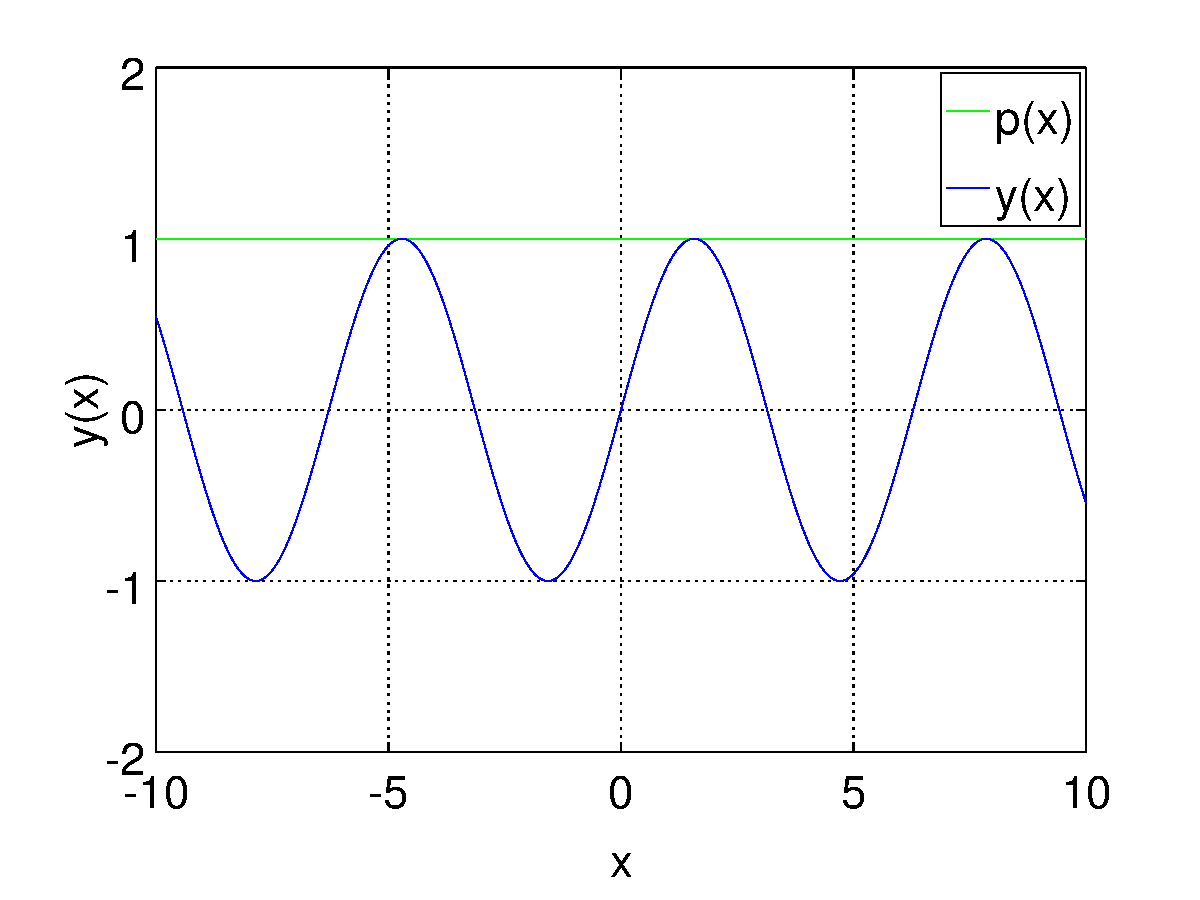
\includegraphics[width=0.5\hsize]{./wellen/images/basicfunctions/sin.pdf}
	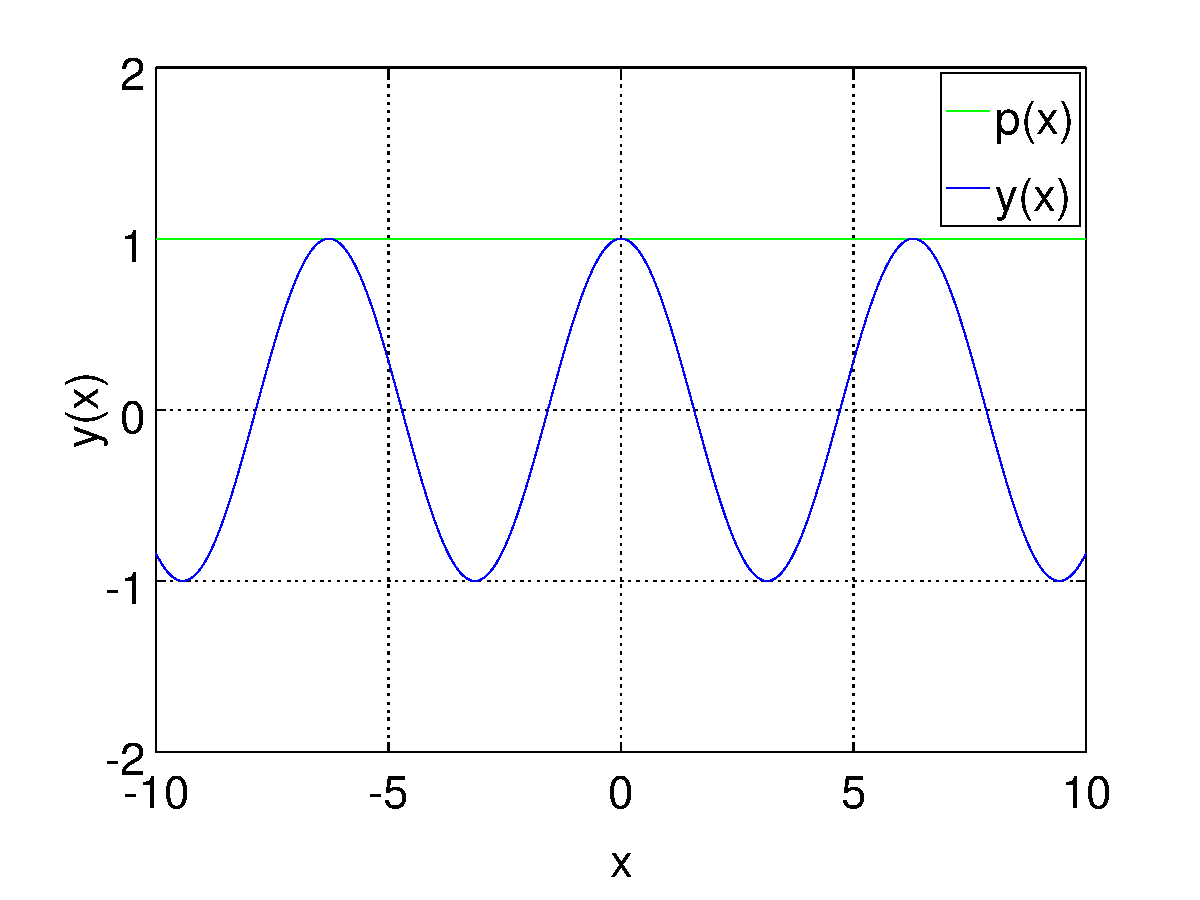
\includegraphics[width=0.5\hsize]{./wellen/images/basicfunctions/cos.pdf}
	\caption{Links $\sin(x)$ und rechts $\cos(x)$.}
	\label{fig:wellen:sin-cos}
\end{figure}

\begin{figure}
	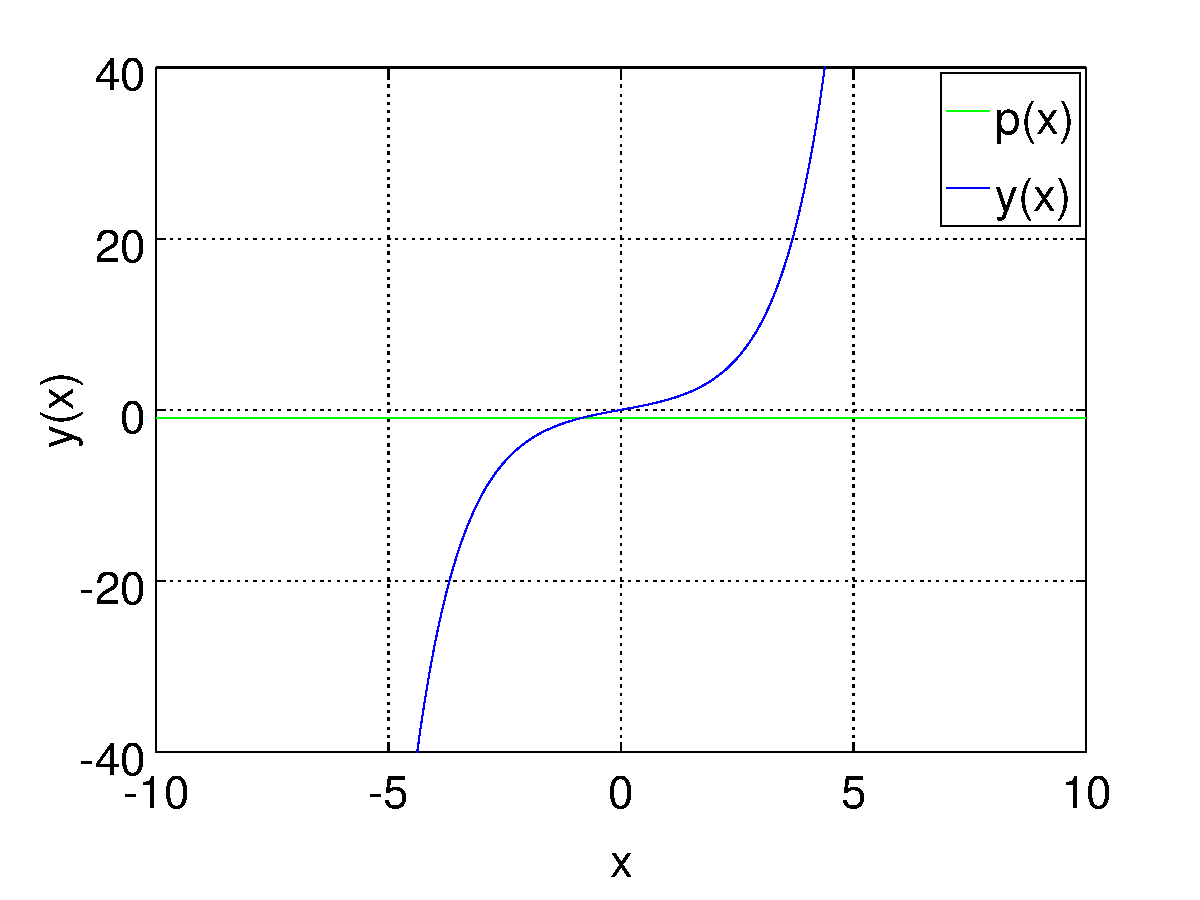
\includegraphics[width=0.5\hsize]{./wellen/images/basicfunctions/sinh.pdf}
	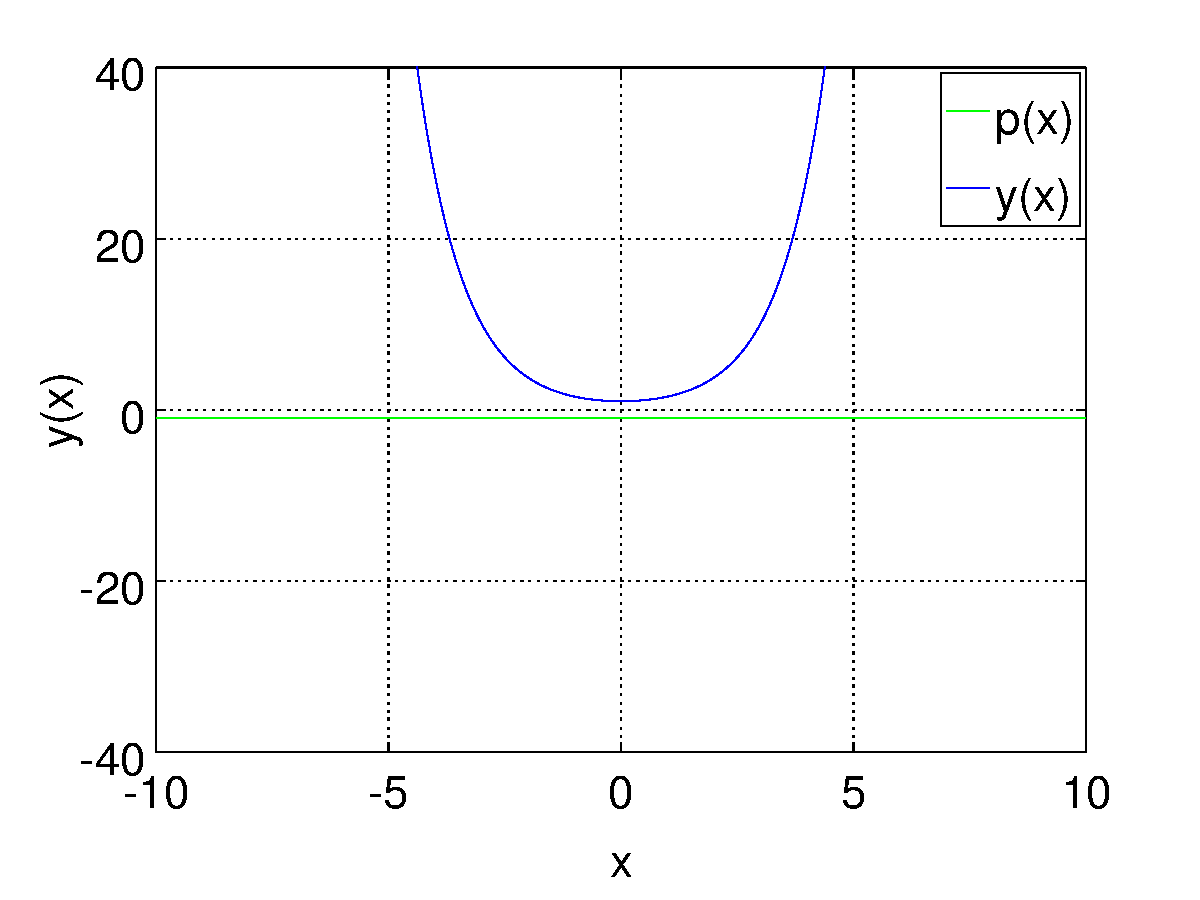
\includegraphics[width=0.5\hsize]{./wellen/images/basicfunctions/cosh.pdf}
	\caption{Links $\sinh(x)$ und rechts $\cosh(x)$.}
	\label{fig:wellen:sinh-cosh}
\end{figure}